% Chapter 2

\chapter{Stato dell'arte} % Write in your own chapter title
\label{Capitolo 2}
\lhead{Capitolo 2. \emph{Stato dell'arte}} % Write in your own chapter title to set the page header

\par
In questo capitolo sar\`{a} descritto lo stato dell'arte riguardanti gli studi e le analisi effettuate relative ad informazioni di tipo geolocalizzato riguardanti gli esseri umani; questa tipologia di dati abbraccia diversi ambiti, tra i quali l'ambito sociale e l'ambito scientifico.
\par
L'interesse che gli accademici che si occupano di sociologia e comportamento umano \`{e} dovuto principalmente al modo in cui gli spostamenti delle persone condizionino le amicizie e relazioni tra loro, ma soprattutto come l'analisi dei dati sia spesso contrastante con l'impressione che hanno le persone stesse dei loro spostamenti, come esposto da Nathan Eagle ed altri in \citep{Reference1}.
\par
Un'altro ambito in cui lo studio di informazioni di tipo geolocalizzato \`{e} quello scientifico, dove si pu\`{o} trovare l'applicazione di diverse discipline matematiche per effettuare l'analisi di dati grezzi; tra queste la teoria dei grafi e la statistica sono sicuramente le maggiormente utilizzate. Gli studiosi che si occupano di scienze sono interessati all'aggregazione dei dati grezzi in dati pi� strutturati, per poter, ad esempio, essere in grado di predirre sia le posizioni delle persone nel futuro, sia le relazioni di amicizia tra gli utenti nel tempo.
\\
Infine, utilizzando i dati strutturati in maniera adeguata, \`{e} possibile creare un sistema di raccomandazione e stimare la similitude tra utenti basandosi solamente su informazioni di tipo geolocalizzato.
\newpage
\section{Ambito sociale}
\par
Lo studio di Nathan Eagle ed altri in \citep{Reference1}, il quale � durato complessivamente nove mesi, si basa su 94 soggetti dello stesso gruppo di lavoro dotati di smartphone che hanno installato al loro interno alcune applicazioni che permettono di registrare ed inviare ad i ricercatori diverse informazioni, tra cui il log delle chiamate, l'identificativo dei dispositivi Bluetooth che sono stati a meno di cinque metri dal soggetto e l'identificativo della cella attraverso la quale lo smartphone riceve il segnale.
\par
Oltre a questi dati analitici, che possiamo definire comportamentali, ad ogni soggetto \`{e} stato chiesto di compilare alcuni questionari mensili che mirano a raccogliere informazioni personali riguardanti le relazioni d'amicizia e la durata approssimativa della vicinanza con altri soggetti; i dati emersi da questi questionari vengono definiti autodichiarati.
\par
L'analisi di tutti i dati raccolti � divisa in tre fasi:
\begin{itemize}
  \item analisi della relazione tra dati comportamentali ed autodichiarati
  \item analisi della presenza di dati comportamentali che caratterizzano l'amicizia
\end{itemize}

\subsection{Relazione tra dati comportamentali ed autodichiarati}
Negli ultimi trent'anni si \`{e} discusso molto sull'affidabilit\`{a} delle misurazioni esistenti per le relazioni, osservando soprattutto che le osservazioni comportamentali sono debolmente correlate con le interazioni riportate dai soggetti; alcuni studi \citep{Reference2} hanno dimostrato come le persone riescono a ricordare meglio le strutture sociali a lungo termine rispetto a quelle nel breve periodo. Si possono riscontrare due diverse tipologie di bias, uno basato sul ricordo degli eventi recenti denominato \emph{recency bias}, l'altro basato sul ricordo degli eventi pi� importanti denominato \emph{salience bias}; attraverso i dati raccolti si pu� quindi assimilare l'effetto di \emph{recency bias} alla quantit�\`{a} di interazioni in un periodo prefissato antecedente al questionario e l'effetto di \emph{salience bias} alla presenza o meno di una relazione di amicizia tra due soggetti.
\par
Attraverso l'incrocio dei dati comportamentali ed autodichiarati \`{e} emerso che la maggiorparte della prossimit� \`{e} misurata \`{e} stata invece dichiarata dal soggetto come non vicinanza; inoltre, quando i due dati non erano in contrasto, il tempo di contatto � sempre stato sovrastimato, essendo la media dei dati comportamentali di 33 minuti al giorno contro la media dei dati autodichiarati di 87 minuti al giorno. Infine si \`{e} osservato che i dati riportati da soggetti che si reputano amici sono molto pi� precisi rispetto ai dati riportati da soggetti che non si considerano amici.

\subsection{Analisi della presenza di dati comportamentali che caratterizzano l'amicizia}
Analizzare i dati comportamentali per evidenziare il grado di relazioni tra due soggetti, come l'amicizia, \`{e} diverso da misurarne la vicinanza; infatti \`{e} plausibile che due persone anche essendo amiche, siano distanti anche per periodi di tempo piuttosto lunghi. Ad ogni modo il contesto, sia spaziale che temporale, pu� aiutare a definire alcuni pattern per la predizione delle amicizie, ad esempio l'aver passato con un'altra persona poche ore un sabato sera in un posto diverso dal luogo di lavoro indica una relazione differente rispetto all'aver passato quattro ore nel luogo di lavoro di un mercoled\`{i} pomeriggio.
\par
In figura ~\ref{fig:Proximity} \`{e} rappresentata graficamente la distribuzione della probabilit� di vicinanza sia all'interno del luogo di lavoro, sia all'esterno, tra persone che si reputano amici reciprocamente, persone tra le quali solamente una delle parti si reputa amica dell'altra parte e persone che non si reputano amici a vicenda; si nota immediatamente come la vicinanza \`{e} pi� probabile tra le prime due categorie di persone, ma, essendo il luogo d'incontro un fattore determinante, si pu\`{o} osservare come la vicinanza misurata all'esterno del luogo di lavoro sia maggiore per chi si reputa amico reciprocamente.

\begin{figure}[htbp]
  \centering
    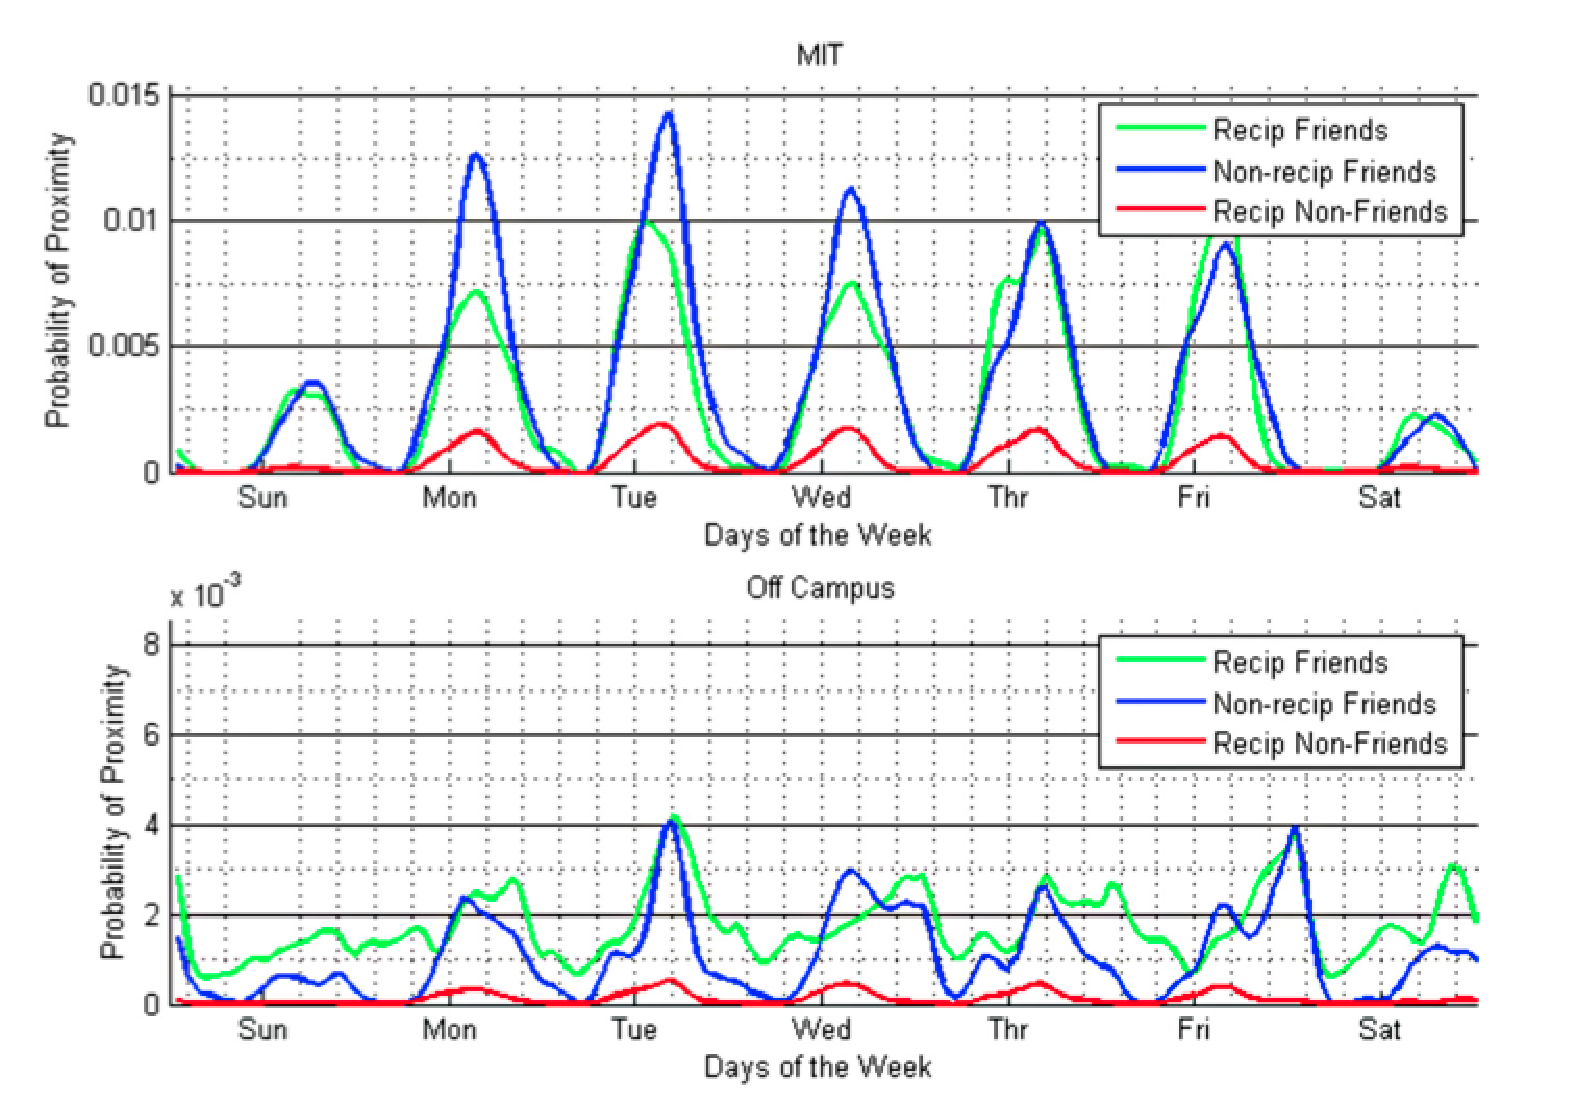
\includegraphics[width=0.8\textwidth]{./Figures/nathan_1.pdf}
    \rule{35em}{0.5pt}
  \caption[Distrubuzione della vicinanza]{Distribuzione della vicinanza nel tempo e nello spazio}
  \label{fig:Proximity}
\end{figure}

Nathan Eagle ed altri hanno successivamente classificato la vicinanza in diverse variabili corrispondenti alla vicinanza all'interno o all'esterno del campus, alla vicinanza di giorno o di notte e alla vicinanza nei giorni lavorativi o nei fine settimana; una fattorizzazione di queste variabili ha evidenziato come esistano solamente due fattori discriminanti, ovvero la vicinanza durante le ore del giorno nel luogo di lavoro e la vicinanza nelle ore serali o nei fine settimana all'esterno del campus. Solamente utilizzando il secondo fattore \`{e} possibile predirre il 96\% percento dei rapporti di non amicizia reciproca ed il 95\% percento dei rapporti di amicizia reciproca, potendo quindi tralasciare i dati autodichiarati di amicizia, quest'ultima risulta stimabile correttamente utilizzando solamente i dati comportamentali.


\section{Ambito scientifico}
\subsection{Predizione delle traiettorie}
\subsection{Predizione delle connessioni tra utenti}
\subsection{Sistema di raccomandazione}
\subsection{Similitude tra utenti}